% 原书 p.101–p.115（PDF p.109–p.123）；本节为第 5 章 5.1 节（Morse 理论）
% 文件顺序：ch05a-s01.tex（本章开头 + 5.1）→ ch05a-s02.tex（5.2）
\chapter{Floer 理论（Floer Theory）}

% >>> p109
Floer 理论是辛几何中最强有力的理论，已被用来导出辛对象的种种同调刚性。视所涉及的
几何对象或动力对象不同，它有若干不同版本。本章将简要介绍为研究哈密顿微分同胚的不动点
而设计的\textbf{哈密顿 Floer 理论}。大多数 Floer 理论都可视为一种\textbf{无穷维 Morse
理论}（$\infty$-dimensional Morse theory），只不过所讨论的空间要么是环路空间，要么是
（某个底辛流形上的）道路空间。一个值得注意的事实是：关于环路空间或道路空间的结果，
可以蕴含底辛流形自身的刚性。Floer 理论的困难始终在于其良定义性，而这通常要靠一套
适当改造过的伪全纯曲线理论来保证。

% [Tutor Note: 易错预警——本章所说的「Floer 理论」默认指哈密顿 Floer 理论（Hamiltonian
% Floer theory）；同一名词在文献中亦指拉格朗日 Floer 理论（Lagrangian Floer theory），
% 两者所对应的环路空间/道路空间与作用量泛函并不相同。阅读后续 5.3–5.5 节时请先确认
% 上下文中的版本。]

\noindent\textbf{本章导读。}本章以有限维 Morse 理论为「玩具模型」逐步搭建 Floer 理论：
5.1 节用 Morse 函数的负梯度流线构造模空间、给出维数公式与紧化，并得到 Morse 链复形与
Morse 同调；5.2 节引入持续模与条形码，把临界值的信息定量化；5.3 节列举辛几何中种种
同调刚性猜想（Arnold 猜想等）；5.4 节把前面的构造搬到无穷维，正式定义哈密顿 Floer
同调；5.5 节讨论 Floer 理论中出现的各种指标（Conley–Zehnder 指标、Maslov 指标等）。

\section{Morse 理论（Morse Theory）}

\begin{keytakeaways}
\begin{itemize}
  \item 几何图像：用 Morse 函数的临界点及其负梯度流线来研究流形 $X$ 的拓扑；
        两条临界点之间的连线段族构成\textbf{模空间} $\mathcal M(x,y)$。
  \item 数学工具：Morse 引理（局部标准形 (5.1)）给出指标；对通有度量，稳定流形与
        不稳定流形横截相交，从而模空间是流形，其维数由指标差 $\ind(x)-\ind(y)$ 决定。
  \item 紧化：流线序列的极限是\textbf{断裂流线}，故模空间可紧化为带角流形，其
        余维 $k$ 分层由 $k$ 次断裂流线给出。
  \item 本节结论：模 $2$ 计数流线得到 Morse 链复形 $(\mathrm{CM}_*,\partial_*)$，
        满足 $\partial^2=0$；所得 Morse 同调 $\mathrm{HM}_*(F,g;\Z_2)\cong H_*(X;\Z_2)$
        与 Morse 函数及度量的选取无关，由此得到 Morse 不等式
        $\#\Crit(F)\geqslant\sum_i b_i(X;\mathbf k)$。
\end{itemize}
\end{keytakeaways}

Morse 理论，或其经典名称「大范围变分法」（calculus of variations in the large，
见 [163]），通过（Morse）函数的临界点来研究流形 $X$ 的拓扑。引入 Morse 理论有若干
途径；本节我们将聚焦于一种相对较新的途径，它基于流轨迹构成的模空间。给定 $X$ 上的
函数 $F$，记 $\Crit(F)$ 为 $F$ 在 $X$ 上的临界点集（即对任意 $p\in\Crit(X)$ 有
$\dd F(p)=0$）。

% [Tutor Note: 原文疑误——括注中写的是 p ∈ Crit(X)，应为 p ∈ Crit(F)：临界点集是函数 F
% 的属性，与空间 X 无关。译文保留原文写法，已在 review_ch05a.md 中记录。]

\begin{wdefn}{5.1.1}
一个 $C^2$ 可微函数 $F$ 称为 \textbf{Morse 函数}，如果在其每个临界点
$p\in\Crit(F)$ 处，$F$ 在 $p$ 的 Hessian 是非退化的。等价地，在 $p$ 附近的局部坐标
$(x_i)_{i=1,\cdots,\dim M}$ 下，相应的矩阵
\[
\left(\frac{\partial^2 F}{\partial x_i\partial x_j}\right)(p)
\]
可逆。
\end{wdefn}

% [Tutor Note: 记号依据——原书定义中流形记作 M，而全章其余地方记作 X（$n$ 维）；此处照
% 原文保留 $\dim M$，不是笔误的翻译。Hessian 非退化即该对称矩阵可逆，等价于 $p$ 是
% $\dd F$ 的非退化零点。]

\begin{wexam}{5.1.1}
取 $X=\R^2$，坐标为 $(x_1,x_2)$。考虑如下函数
\[
F(x_1,x_2)=x_1^2-x_2^2,\qquad\text{则}\quad
\left(\frac{\partial^2 F}{\partial x_i\partial x_j}\right)(0)
=\begin{pmatrix}2&0\\0&-2\end{pmatrix},
\]
% >>> p110
它非退化。由于 $0\in\R^2$ 是 $F$ 的唯一临界点，故由定义 5.1.1，这个 $F$ 是 Morse
函数。再考虑如下函数
\[
G(x_1,x_2)=x_1^3-x_2^2,\qquad\text{则}\quad
\left(\frac{\partial^2 G}{\partial x_i\partial x_j}\right)(0)
=\begin{pmatrix}0&0\\0&-2\end{pmatrix},
\]
它退化。因此由定义 5.1.1，$G$ 不是 Morse 函数。\hfill$//$
\end{wexam}

下面两个事实（分别取自 [156] 中的引理 2.2，以及 [102] 第 1 章第 7 节末尾附近的
定理）大致说明：Morse 函数是一般光滑函数的良好逼近，并且具有良好而可控的局部性质。

\par\medskip\noindent\hangindent=2.2em\hangafter=1
\textbf{事实 5.1.1}\quad 设 $F$ 是 $n$ 维紧流形 $X$ 上的任意 Morse 函数，
$p\in\Crit(F)$，则存在该临界点 $p$ 附近的局部坐标 $x=(x_1,\cdots,x_n)$，使得
$x(p)=(0,\cdots,0)$ 且
\begin{equation}\tag{5.1}
F(x)=F(p)-\sum_{i=1}^{k}x_i^2+\sum_{j=k+1}^{n}x_j^2.
\end{equation}

% [Tutor Note: 含糊点拨——事实 5.1.1 就是 Morse 引理。证明分两步：先对 $F$ 在 $p$ 处作
% Taylor 展开，再用「沿直线积分」的技巧把二次项写成 $x^{\mathsf T}H(x)x$ 的形式（$H(x)$
% 为对称矩阵族且 $H(p)$ 为 Hessian），最后用 Sylvester 惯性定理把 $H(p)$ 对角化为
% $(-1,\cdots,-1,+1,\cdots,+1)$ 并作坐标变换。教材通常把它放在「Morse 引理」条目下，
% 可参看 Milnor, \emph{Morse Theory}, 第 2 节。原文给出两个文献 [156]、[102]，其中 [156]
% 的引理 2.2 即此引理。]

这一事实使我们能把 Morse 函数 $F$ 在 $p$ 处的\textbf{指标}（index）定义为 (5.1) 中
单项式 $\{x_i^2\}_{i=1,\cdots,n}$ 里负项的个数。值得注意的是，$F$ 在 $p$ 处的指标与
$p$ 附近局部坐标的选取无关，记作 $\ind_F(p)$，或在无需强调 Morse 函数时简记作
$\ind(p)$。

% [Tutor Note: 易错预警——指标等于 Hessian 的\emph{负}特征值个数（不是正特征值个数，
% 也不是非零特征值个数）：局部极小点指标为 $0$，局部极大点指标为 $n$。指标与坐标无关
% 是 Sylvester 惯性定理的直接推论。后文所有维数公式中的 $\ind$ 都按此约定。]

\par\medskip\noindent\hangindent=2.2em\hangafter=1
\textbf{事实 5.1.2}\quad 在紧光滑流形 $X$ 上，全体 Morse 函数的集合在
$C^\infty(X;\R)$（即 $X$ 上全体光滑函数之集）中稠密。

该事实允许用 Morse 函数逼近任意光滑函数。这是一个相当方便的性质：一般的光滑函数可能
有非常退化的临界点集，通常难以处理；而对 Morse 函数，我们本质上只与点打交道。

% [Tutor Note: 含糊点拨——稠密性的标准证明用 Sard 定理（或更一般地，用横截性定理）：
% 对 $F$ 加一个足够小、足够通有的扰动即可消除临界点的退化。Morse 理论中因此总可假设
% $F$ 的临界值互不相同、临界点有限；本书后文（例如 Morse 链复形的构造）默认如此。]

\begin{wrem}{5.1.1}
注意，对光滑流形 $X$ 上的 Morse 函数 $F$，临界点集 $\Crit(F)$ 是 $X$ 的无处稠密
子集。事实上，临界点总是孤立的。
\end{wrem}

% [Tutor Note: 易错预警——「孤立」来自 Hessian 可逆：把反函数定理用于 $\dd F$ 可知每个
% 临界点有邻域使 $\dd F$ 仅在 $p$ 处为零。再结合 $X$ 紧，可得 $\Crit(F)$ 为有限集，
% 这一步在 5.1 节末尾构造链复形时反复用到。]

现在固定 $X$ 上的一个度量 $g$。对 Morse 函数 $F:X\to\R$，考虑如下常微分方程
\begin{equation}\tag{5.2}
\frac{\dd u(t)}{\dd t}=-\nabla_g F(u(t)),
\end{equation}
其中 $u:\R\to X$ 是 $t$ 的光滑函数。(5.2) 的任一解就是 $F$（关于度量 $g$）的
\textbf{负梯度流}，而集合 $\{u(t)\}_{t\in\R}$ 称为一条\textbf{负梯度流线}。为解
(5.2)，还需要初始条件。由于 $t$ 取自整个 $\R$，且该微分方程可以按时间 $t$ 反向求解，
我们需要
% >>> p111
两个条件，分别处理 $t=-\infty$ 与 $t=\infty$ 两端。由一条分析事实（见 [132] 中的
引理 6.4.7），我们令 $u(-\infty)=x$、$u(\infty)=y$，其中 $x,y\in\Crit(F)$。

% [Tutor Note: 含糊点拨——沿 (5.2) 的解有 $\frac{\dd}{\dd t}F(u(t))
% =-|\nabla_g F(u(t))|^2\leqslant 0$，故 $F$ 沿流线不增（这正是练习 5.1.1 的提示）；
% 在非临界点处严格递减。端点极限 $u(\pm\infty)$ 的存在性以及「极限必为临界点」需要
% 能量估计与紧性论证（所引 [132] 的引理 6.4.7 即此类分析事实）。在 5.4 节的 Floer
% 理论中，对应的对象是有限能量伪全纯曲线，其端点极限存在性正是紧性理论的核心。]

接下来沿用上面的记号，考虑模空间
\[
\widetilde{\mathcal M}_{F,g}(x,y):=
\left\{u:\R\to X\ \middle|\
\begin{array}{l}
\dfrac{\dd u(t)}{\dd t}=-\nabla_g F(u(t)),\\[6pt]
u(-\infty)=x\ \text{且}\ u(\infty)=y
\end{array}\right\}.
\]
第一个观察是：每个 $u\in\widetilde{\mathcal M}_{F,g}(x,y)$ 上都存在一个 $\R$-作用，
由 $s\cdot u(t):=u(s+t)$（$s\in\R$）给出，即 $\R$-平移。于是显然 $\R\cdot u$ 也落在
$\widetilde{\mathcal M}_{F,g}(x,y)$ 中。因此，更有效的是考虑如下\textbf{约化模空间}
\begin{equation}\tag{5.3}
\mathcal M_{F,g}(x,y):=\widetilde{\mathcal M}_{F,g}(x,y)/\R\text{-平移}.
\end{equation}

% [Tutor Note: 易错预警——(5.3) 中的 $\R$-作用是自由作用：若 $s\cdot u=u$ 对某个 $s\ne0$
% 成立，则 $u$ 关于 $t$ 周期，这与 $u(-\infty)=x\ne y=u(\infty)$ 矛盾。因此每条流线
% 的 $\R$-轨道是一维的，约化模空间的维数比 $\widetilde{\mathcal M}$ 少 $1$；这一点在
% 命题 5.1.1 的公式 $\dim\mathcal M=\ind(x)-\ind(y)-1$ 中体现出来。]

\begin{wexer}{5.1.1}
设 $F$ 是光滑流形 $(X,g)$ 上的 Morse 函数。证明：对任意临界点 $x\in\Crit(F)$，
模空间 $\widetilde{\mathcal M}_{F,g}(x,x)$ 只含 $x$ 处的常值流。特别地，商模空间
$\mathcal M_{F,g}(x,x)$ 只含一个点。（提示：Morse 函数 $F$ 沿流线
$\{u(t)\}_{t\in\R}$ 不增。）
\end{wexer}

上述练习蕴含：对两个不同的临界点 $x,y\in\Crit(F)$，若约化模空间
$\mathcal M_{F,g}(x,y)$ 的维数为零，则原模空间 $\widetilde{\mathcal M}_{F,g}(x,y)$
的维数至多为 $1$（假定其流形结构成立，参见事实 5.1.1）。

% [Tutor Note: 易错预警——练习 5.1.1 的要点是：若 $F$ 沿非常值流线严格递减，则
% $u$ 不可能有 $u(-\infty)=u(\infty)$；换成严格递减的论证需要「非临界点处
% $|\nabla_g F|^2>0$」。另注意「维数为零的约化模空间」与「非空」是两回事，后者
% 要单独讨论（见本节命题 5.1.1 之后的结论）。]

下面我们来算几个例子。这些例子将展示（用 Morse 函数表达的）可计算性。

\begin{wexam}{5.1.2}
取 $X=S^1\subset\R^2$ 为图 5.1 所示的标准圆周。对任意点 $p=(x_p,y_p)\in S^1$，
考虑 Morse 函数 $F(p)=y_p$，即高度函数。在极坐标 $(\cos(t),\sin(t))\in S^1$，
$t\in[0,2\pi)$ 下，可以改写 $F(\cos(t),\sin(t))=\sin(t)$，从而
$\dfrac{\partial F}{\partial t}=\cos(t)$。故 $F$ 的临界点是 $S^1$ 的南极与北极，
分别记作 $p_0$ 与 $p_1$。

\begin{figure}[htbp]
  \centering
  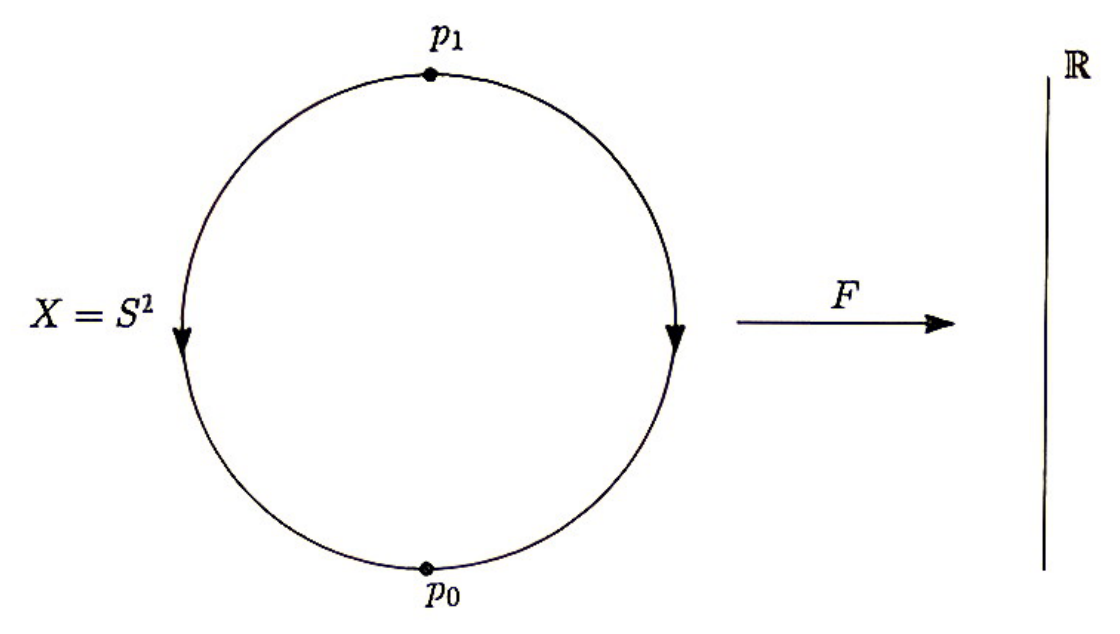
\includegraphics[width=0.62\linewidth]{figures/fig_p111_1.png}
  \caption*{图 5.1\quad 标准 $S^1\subset\R^2$ 上的高度函数（原书 p.103,
  Figure 5.1；PDF p.111）}
\end{figure}

% >>> p112
在 $p_0$ 附近，$F$ 的局部表达式为 $F(x)=x^2$，故 $\ind(p_0)=0$。在 $p_1$ 附近，
$F$ 的局部表达式为 $F(x)=-x^2$，故 $\ind(p_1)=1$。

取标准度量 $g$（由图 5.1 中的嵌入从 $\R^2$ 诱导），模空间
$\widetilde{\mathcal M}_{F,g}(p_1,p_0)$ 由两族 $\R$-参数化的、从 $p_1$ 到 $p_0$ 的
流线组成，其方向分别为顺时针与逆时针。故约化模空间
$\mathcal M_{F,g}(p_1,p_0)$ 含两个元素。\hfill$//$
\end{wexam}

% [Tutor Note: 易错预警——此例中 $\dim\widetilde{\mathcal M}=\ind(p_1)-\ind(p_0)=1$，
% 即每条流线恰有一个 $\R$-平移参数；约化后「两个元素」对应两条方向不同的流线，
% 而不是「两族」。若用 $\Z_2$ 系数计数，这两条流线的贡献 $1+1=0$，这也预示了
% $S^1$ 的 Morse 同调中 $\partial_1=0$。]

\begin{wexam}{5.1.3}
取 $X$ 为 $\R^2$ 中的心形圆周（见图 5.2）。与例 5.1.2 类似，考虑高度函数
$F(p)=y_p$，$p\in X$。容易看出 $F$ 是 Morse 函数，且在 $X$ 上有四个临界点，记作
$p_0,p_1,q_0,q_1$。可以算出
\[
\ind(p_0)=\ind(q_0)=0,\qquad \ind(p_1)=\ind(q_1)=1.
\]

盯着图 5.2 便知，模空间 $\widetilde{\mathcal M}_{F,g}(p_1,p_0)$ 只含一族
$\R$-参数化的流线；对 $\widetilde{\mathcal M}_{F,g}(q_1,p_0)$、
$\widetilde{\mathcal M}_{F,g}(p_1,q_0)$ 与 $\widetilde{\mathcal M}_{F,g}(q_1,q_0)$
同样如此。然而，从 $q_0$ 到 $p_0$ 没有流线（否则 Morse 函数 $F$ 必须经过 $p_1$ 或
$q_1$，其值将增大）。因此 $\mathcal M_{F,g}(q_0,p_0)=\varnothing$。类似地，有
$\mathcal M_{F,g}(p_1,q_1)=\varnothing$。\hfill$//$
\end{wexam}

% [Tutor Note: 含糊点拨——「没有流线」的理由是流线沿 $F$ 严格递减：从 $q_0$ 下行的
% 流线若到达 $p_0$，则 $F$ 必须先经过 $p_1$ 或 $q_1$ 的高度层，而这两处的 $F$ 值
% 大于 $F(q_0)$，矛盾。这里用到的正是 $X$ 为一维流形、指标只有 $0,1$ 两种的事实；
% 对高维流形，指标只能保证 $\mathcal M(x,y)$ 的期望维数为 $\ind(x)-\ind(y)-1$，
% 不能直接断定其非空或为空。]

\begin{figure}[htbp]
  \centering
  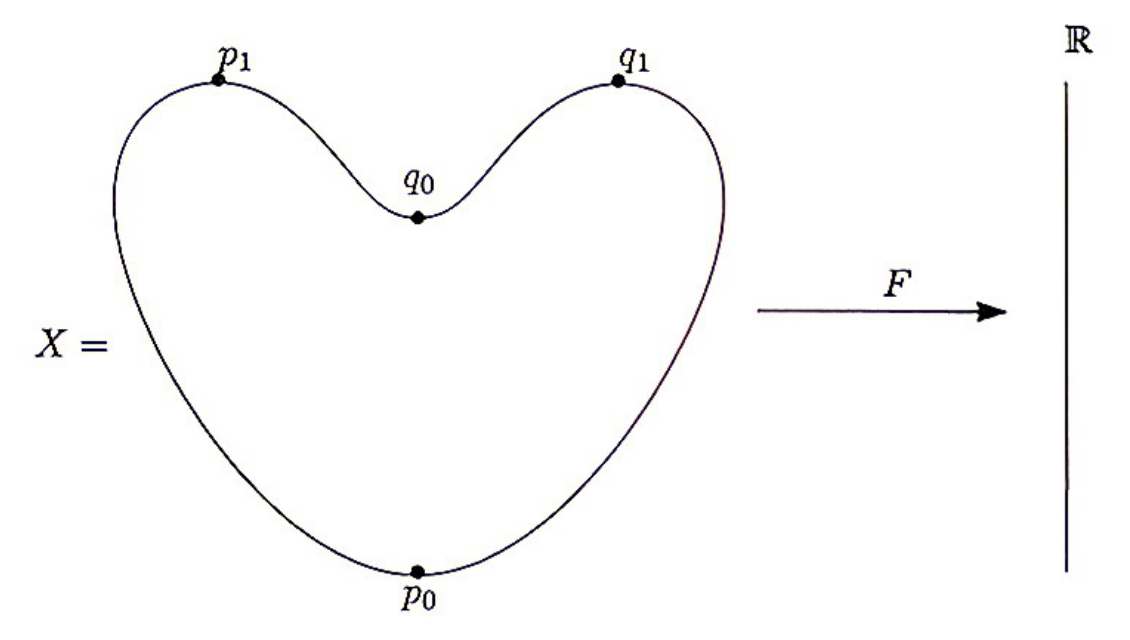
\includegraphics[width=0.62\linewidth]{figures/fig_p112_1.png}
  \caption*{图 5.2\quad $\R^2$ 中心形圆周 $X$ 上的高度函数（原书 p.104,
  Figure 5.2；PDF p.112）}
\end{figure}

\begin{wexam}{5.1.4}（[183] 中的练习 1.16）
取 $X=S^1\times S^1=\R/(2\pi\Z)\times\R/(2\pi\Z)$，即 $\R^3$ 中的标准 2-环面，
考虑函数 $F(t_1,t_2)=\sin(t_1)+\sin(t_2)$，其中
$(t_1,t_2)\in\R/(2\pi\Z)\times\R/(2\pi\Z)$（见图 5.3）。该 $F$ 有四个临界点
\[
\begin{aligned}
p_2&=\left(\frac{\pi}{2},\frac{\pi}{2}\right),&\quad
p_1&=\left(\frac{3\pi}{2},\frac{\pi}{2}\right),\\
q_1&=\left(\frac{\pi}{2},\frac{3\pi}{2}\right),&\quad
p_0&=\left(\frac{3\pi}{2},\frac{3\pi}{2}\right).
\end{aligned}
\]
注意，该函数 $F$ 是例 5.1.2 中的高度函数在 2-环面 $X$ 的每个圆周因子上的（外）积。
而且，它确实是 Morse 函数，这由

% >>> p113
\begin{figure}[htbp]
  \centering
  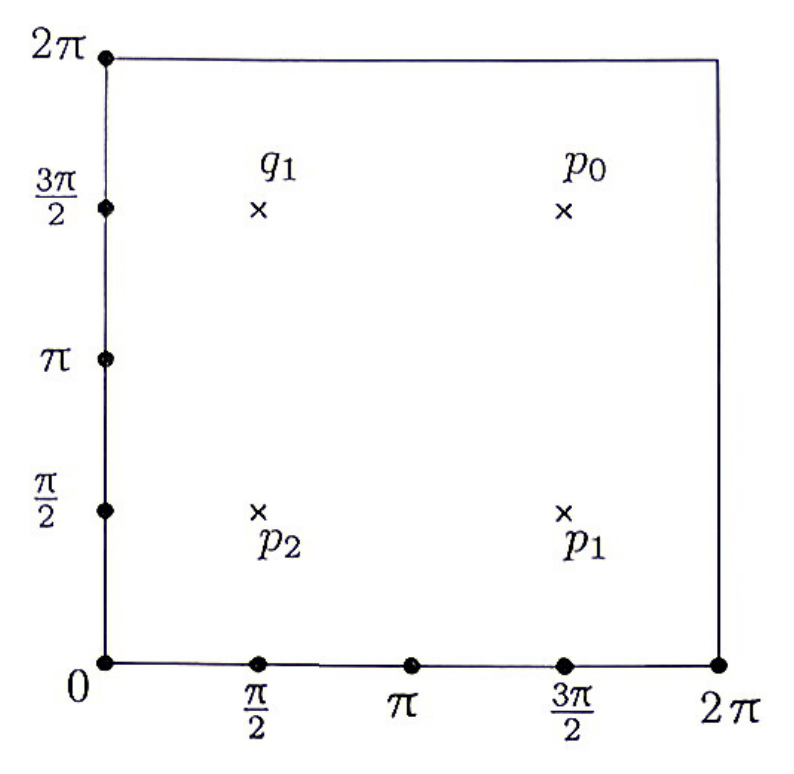
\includegraphics[width=0.40\linewidth]{figures/fig_p113_1.png}
  \caption*{图 5.3\quad 2-环面 $S^1\times S^1$ 上高度函数之积（原书 p.105,
  Figure 5.3；PDF p.113）}
\end{figure}

定义 5.1.1 可得，因为可以算出各临界点处作为 $F$ 的 Hessian 的矩阵：
\begin{align*}
\left(\frac{\partial^2 F}{\partial t_1\partial t_2}\right)\bigg|_{p_0}
&=\begin{pmatrix}-\sin(t_1)&0\\0&-\sin(t_2)\end{pmatrix}\bigg|_{p_0}
=\begin{pmatrix}1&0\\0&1\end{pmatrix},\\
\left(\frac{\partial^2 F}{\partial t_1\partial t_2}\right)\bigg|_{p_1}
&=\begin{pmatrix}-\sin(t_1)&0\\0&-\sin(t_2)\end{pmatrix}\bigg|_{p_1}
=\begin{pmatrix}1&0\\0&-1\end{pmatrix},\\
\left(\frac{\partial^2 F}{\partial t_1\partial t_2}\right)\bigg|_{q_1}
&=\begin{pmatrix}-\sin(t_1)&0\\0&-\sin(t_2)\end{pmatrix}\bigg|_{q_1}
=\begin{pmatrix}-1&0\\0&1\end{pmatrix},\\
\left(\frac{\partial^2 F}{\partial t_1\partial t_2}\right)\bigg|_{p_2}
&=\begin{pmatrix}-\sin(t_1)&0\\0&-\sin(t_2)\end{pmatrix}\bigg|_{p_2}
=\begin{pmatrix}-1&0\\0&-1\end{pmatrix}.
\end{align*}
同时，可以读出各临界点的指标
\[
\ind(p_0)=0,\qquad \ind(p_1)=\ind(q_1)=1,\qquad \ind(p_2)=2.
\]
取 $X$ 上的标准度量 $g$（即例 5.1.2 中 $S^1\subset\R^2$ 上标准度量的乘积），则
\[
\nabla_g F=\left(\frac{\partial F}{\partial t_1},\frac{\partial F}{\partial t_2}\right)
=(\cos(t_1),\cos(t_2)).
\]
若 $u:\R\to X$ 是梯度流，并记 $u=(u_1(t),u_2(t))$，则 (5.2) 化为
\[
\begin{cases}
\dfrac{\dd u_1(t)}{\dd t}=-\cos(u_1(t)),\\[8pt]
\dfrac{\dd u_2(t)}{\dd t}=-\cos(u_2(t)).
\end{cases}
\]
给定初始条件 $t(-\infty)=p_2$ 与 $t(+\infty)=p_0$，可以验证模空间
$\mathcal M_{F,g}(p_2,p_0)$ 中有大量（未参数化的）解，其相应的
% >>> p114
负流轨迹几乎填满图 5.4 中的每个小开方块（图 5.4 是图 5.3 在 $p_2$ 处居中后的变形图）。
注意，由 2-环面的构造，图 5.3 中的四个顶点都是 $p_0$。

% [Tutor Note: 原文疑误——此句原文写作「Given the initial condition $t(-\infty)=p_2$ and
% $t(+\infty)=p_0$」，其中的 $t$ 应为流 $u$：$t$ 是定义域参数，$u(\pm\infty)$ 才是
% 流线的端点。译文照原文保留，已在 review_ch05a.md 记录。]

\begin{figure}[htbp]
  \centering
  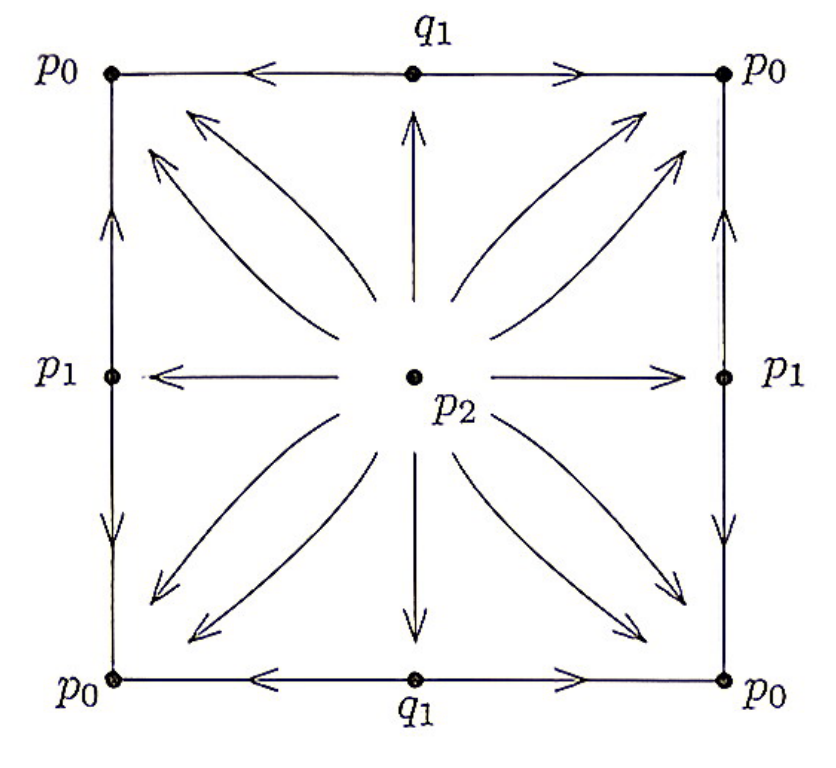
\includegraphics[width=0.44\linewidth]{figures/fig_p114_1.png}
  \caption*{图 5.4\quad $S^1\times S^1$ 中从 $p_2$ 到 $p_0$ 的流线（原书 p.106,
  Figure 5.4；PDF p.114）}
\end{figure}

有趣的是，考虑形如 $u(t)=(\pi/2,u_2(t))$ 的解，其中 $u_2(t)$ 由上面第二个方程解出；
则相应的曲线不贡献于模空间 $\mathcal M_{F,g}(p_2,p_0)$，因为它最终停在 $q_1$。
类似地，形如 $u(t)=(u_1(t),3\pi/2)$ 的解，其中 $u_1$ 由上面第二个方程解出，从 $q_1$
出发并走向 $p_0$；它同样不贡献于模空间 $\mathcal M_{F,g}(p_2,p_0)$（因为它的起点不对）。
但这两个解「拼」在一起，构成一条（在 $q_1$ 处断裂的）从 $p_2$ 到 $p_0$ 的流线。\hfill$//$
\end{wexam}

% [Tutor Note: 原文疑误——第二句中「$u_1$ 由上面第二个方程解出」应为「第一个方程」
% （即 $\dd u_1/\dd t=-\cos u_1$），因为 $u_1$ 只出现在第一个方程中。译文照原文，
% 已记入 review_ch05a.md。另注意「两个解拼起来」得到的是极限中的\emph{断裂流线}，
% 它不在 $\mathcal M_{F,g}(p_2,p_0)$ 内，而属于其紧化（见 5.1 节后半）。]

由以上各例，我们看到两个奇特现象。
\begin{enumerate}[label=(\roman*)]
  \item 当 $\mathcal M_{F,g}(p,q)=\varnothing$ 时，似乎总有 $\ind(p)\leqslant\ind(q)$。
        参见例 5.1.3 末尾的模空间 $\mathcal M_{F,g}(q_0,p_0)$ 与
        $\mathcal M_{F,g}(p_1,q_1)$。
  \item 模空间 $\mathcal M_{F,g}(p,q)$ 可能不是（序列）紧的。参见例 5.1.4 中的模空间
        $\mathcal M_{F,g}(p_2,p_0)$。
\end{enumerate}
对 (i) 与 (ii) 的解释将涉及 Morse 理论中模空间的深层结构性质。

\begin{wprop}{5.1.1}
设 $F$ 是光滑流形 $X$ 上的 Morse 函数。对通有的度量 $g$ 与任意不同的
$x,y\in\Crit(F)$，模空间 $\widetilde{\mathcal M}_{F,g}(x,y)$ 是 $X$ 的子流形，且
\[
\dim\widetilde{\mathcal M}_{F,g}(x,y)=\ind(x)-\ind(y).
\]
特别地，当 $x\ne y$ 时，
\[
\dim\mathcal M_{F,g}(x,y)=\ind(x)-\ind(y)-1.
\]
\end{wprop}

% [Tutor Note: 易错预警——维数公式的符号与流的方向绑定：这里用的是\emph{负}梯度流
% $\dd u/\dd t=-\nabla_g F$，故 $\widetilde{\mathcal M}(x,y)$ 的维数是
% $\ind(x)-\ind(y)$（从高指标流向低指标）。若改用正梯度流，则公式中指标差反号。
% 另注意 $\dim\widetilde{\mathcal M}$ 是 Fredholm 指标意义下的「期望维数」，
% 通有度量下实际维数等于期望维数，这正是横截性的作用。]

为证明此命题，需要如下记号。设 $x$ 是 $F$ 的临界点。
% >>> p115
定义 $x$ 的\textbf{稳定流形}（关于 Morse 函数 $F$ 与度量 $g$）为
\[
W^s(x):=\left\{a\in X\ \middle|\
\begin{array}{l}
a\ \text{位于 (5.2) 的一条负梯度流线 }u(t)\text{ 上},\\
\text{使得}\ \lim_{t\to\infty}u(t)=x
\end{array}\right\},
\]
而 $x$ 的\textbf{不稳定流形}为
\[
W^u(x):=\left\{a\in X\ \middle|\
\begin{array}{l}
a\ \text{位于 (5.2) 的一条负梯度流线 }u(t)\text{ 上},\\
\text{使得}\ \lim_{t\to-\infty}u(t)=x
\end{array}\right\}.
\]
例如在例 5.1.2 中，有 $W^s(p_0)=X\setminus\{p_1\}$ 与
$W^u(p_1)=X\setminus\{p_0\}$。

\begin{wproof}[命题 5.1.1 的证明（略证）]
稳定流形与不稳定流形都是 $X$ 的子流形。此外，对任意 $x\in\Crit(F)$，有维数计算
\[
\dim W^u(x)=\operatorname{codim}W^s(x)=\ind(x).
\]
对通有的度量 $g$ 与两个不同的临界点 $x,y\in\Crit(F)$，子流形 $W^u(x)$ 与
$W^s(y)$ 横截相交，于是
\[
\operatorname{codim}\left(W^u(x)\cap W^s(y)\right)
=\operatorname{codim}W^u(x)+\operatorname{codim}W^s(y).
\]
可以把 $\widetilde{\mathcal M}_{F,g}(x,y)$ 与 $W^u(x)\cap W^s(y)$ 等同起来。因此
$\widetilde{\mathcal M}_{F,g}(x,y)$ 是 $X$ 的子流形，且维数为
\[
\dim\widetilde{\mathcal M}_{F,g}(x,y)
=\dim\left(W^u(x)\cap W^s(y)\right)=\ind(x)-\ind(y),
\]
证毕。
\end{wproof}

% [Tutor Note: 含糊点拨——这段「略证」省略了三件事：(1) $W^u(x)$、$W^s(y)$ 是子流形，
% 这来自稳定流形定理（在临界点附近把 (5.2) 线性化为 $\dot v=-H(p)v$，再用
% Hartman–Grobman 型论证）；(2) 横截性可对度量 $g$ 用 Sard–Smale 定理取通有 $g$
% 得到（即 Morse–Smale 条件）；(3) 「模空间 = 稳定流形与不稳定流形之交」是因为流线
% 由其上任一点唯一确定。Floer 理论中对应的线性化算子是 Fredholm 算子，但其横截性
% 不能仅靠「对度量取通有」得到，需要正则化或虚拟基本类技术——这正是 Floer 理论
% 比有限维 Morse 理论困难的地方。]

由命题 5.1.1 可推出如下直接结论。
\begin{enumerate}[label=(\roman*)]
  \item 若 $\ind(x)-\ind(y)\geqslant1$，则 $\widetilde{\mathcal M}_{F,g}(x,y)$ 与
        $\mathcal M_{F,g}(x,y)$ 非空。
  \item 特别地，若 $\ind(x)-\ind(y)=1$，则 $\mathcal M_{F,g}(x,y)$ 的维数为零，
        故其中元素可以看作离散的点。
  \item 若 $x\ne y$ 但 $\ind(x)=\ind(y)$，则 $\widetilde{\mathcal M}_{F,g}(x,y)$
        为空（参见例 5.1.3）。
\end{enumerate}

% [Tutor Note: 易错预警——注意 (i) 与 (iii) 的逻辑地位不同。(iii) 有直接证明：若
% $\widetilde{\mathcal M}(x,y)$ 非空，取其元素 $u$，则 $\R$-轨道 $\{s\cdot u\}_{s\in\R}$
% 是 $\widetilde{\mathcal M}(x,y)$ 中一条一维子集，故
% $\dim\widetilde{\mathcal M}(x,y)\geqslant1$，由命题 5.1.1 即得
% $\ind(x)>\ind(y)$。反之，(i) 的「非空」并不是维数公式的直接推论——维数公式只给出
% 模空间的（期望）维数，不保证其非空。使用 (i) 时需要另行论证（例如在具体例子中
% 直接构造流线）。]

接下来我们考察模空间 $\widetilde{\mathcal M}_{F,g}(x,y)$ 或
$\mathcal M_{F,g}(x,y)$ 的紧性。如我们所见，它们一般不是紧的。但我们可以通过不断
添加负梯度流线序列的「极限」来紧化它们。例如，由例 5.1.4 最后一段可见，一个额外的
「极限」可能来自断裂流线，即一条从 $p_2$ 到 $q_1$ 的流线与一条从 $q_1$ 到 $p_0$ 的
流线之并（在 $q_1$ 处转接）。另外，由对称性，它也可能来自从 $p_2$ 到 $p_1$ 的流线
与从 $p_1$ 到 $p_0$ 的流线之并（在 $p_1$ 处转接）。示意图见图 5.5 左图。一般来说，
这些「极限」就是可能经过若干临界点的\textbf{断裂流线}。为了描述模空间的紧化，
让我们引入一个推广光滑带边流形概念的概念。

% >>> p116
\begin{figure}[htbp]
  \centering
  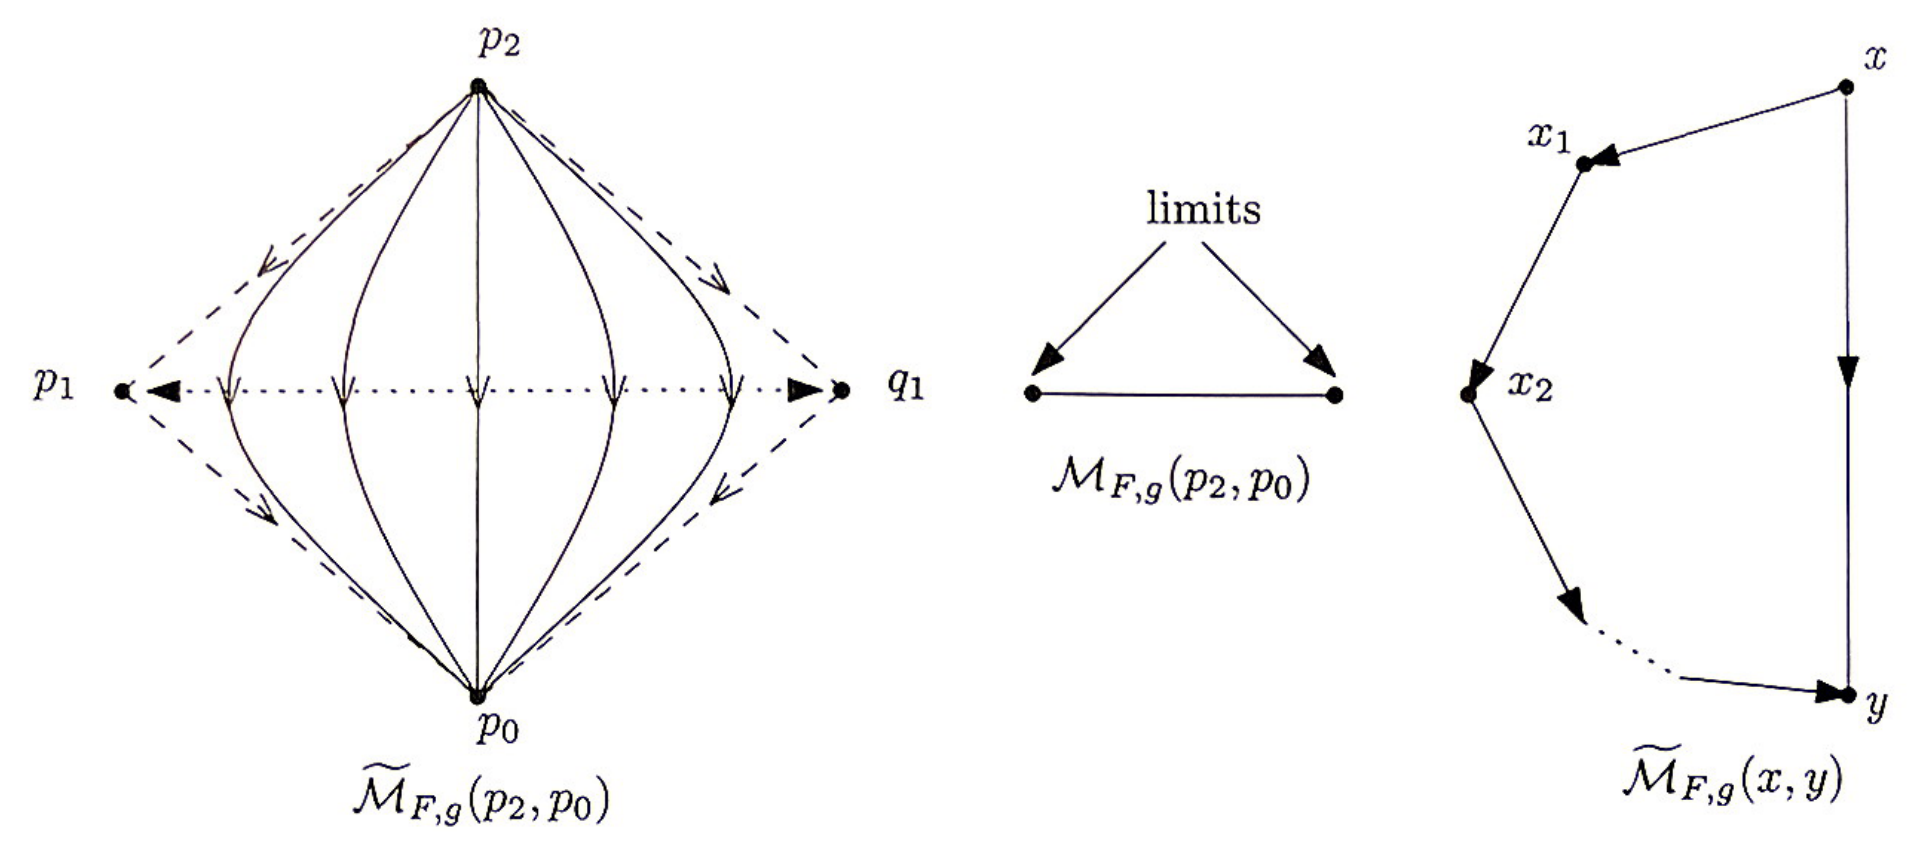
\includegraphics[width=0.95\linewidth]{figures/fig_p116_1.png}
  \caption*{图 5.5\quad 模空间的紧化（原书 p.108, Figure 5.5；PDF p.116）}
\end{figure}

\begin{wdefn}{5.1.2}\ [41,68,142]
一个 $n$ 维\textbf{光滑带角流形}（smooth manifold with corners）$M$ 是一个第二
可数的 Hausdorff 空间，使得对任意 $x\in M$，存在 $x$ 的一个邻域同胚于
$\R^{n-k}\times[0,\infty)^k$ 的某个开子集（其中 $0\leqslant k\leqslant n$），且
转移映射是光滑的（见图 5.6）。
\end{wdefn}

% [Tutor Note: 术语/记号依据——「带角流形」即 manifold with corners，与「带边流形」
% （manifold with boundary，对应 $k\leqslant1$）不同：$k$ 可大于 $1$，此时出现
% 「角」。本书用 $k$ 记录角的重数，$k=0$ 的部分是内部、$k=1$ 是通常的边、$k\geqslant2$
% 是更高余维的角。]

\begin{figure}[htbp]
  \centering
  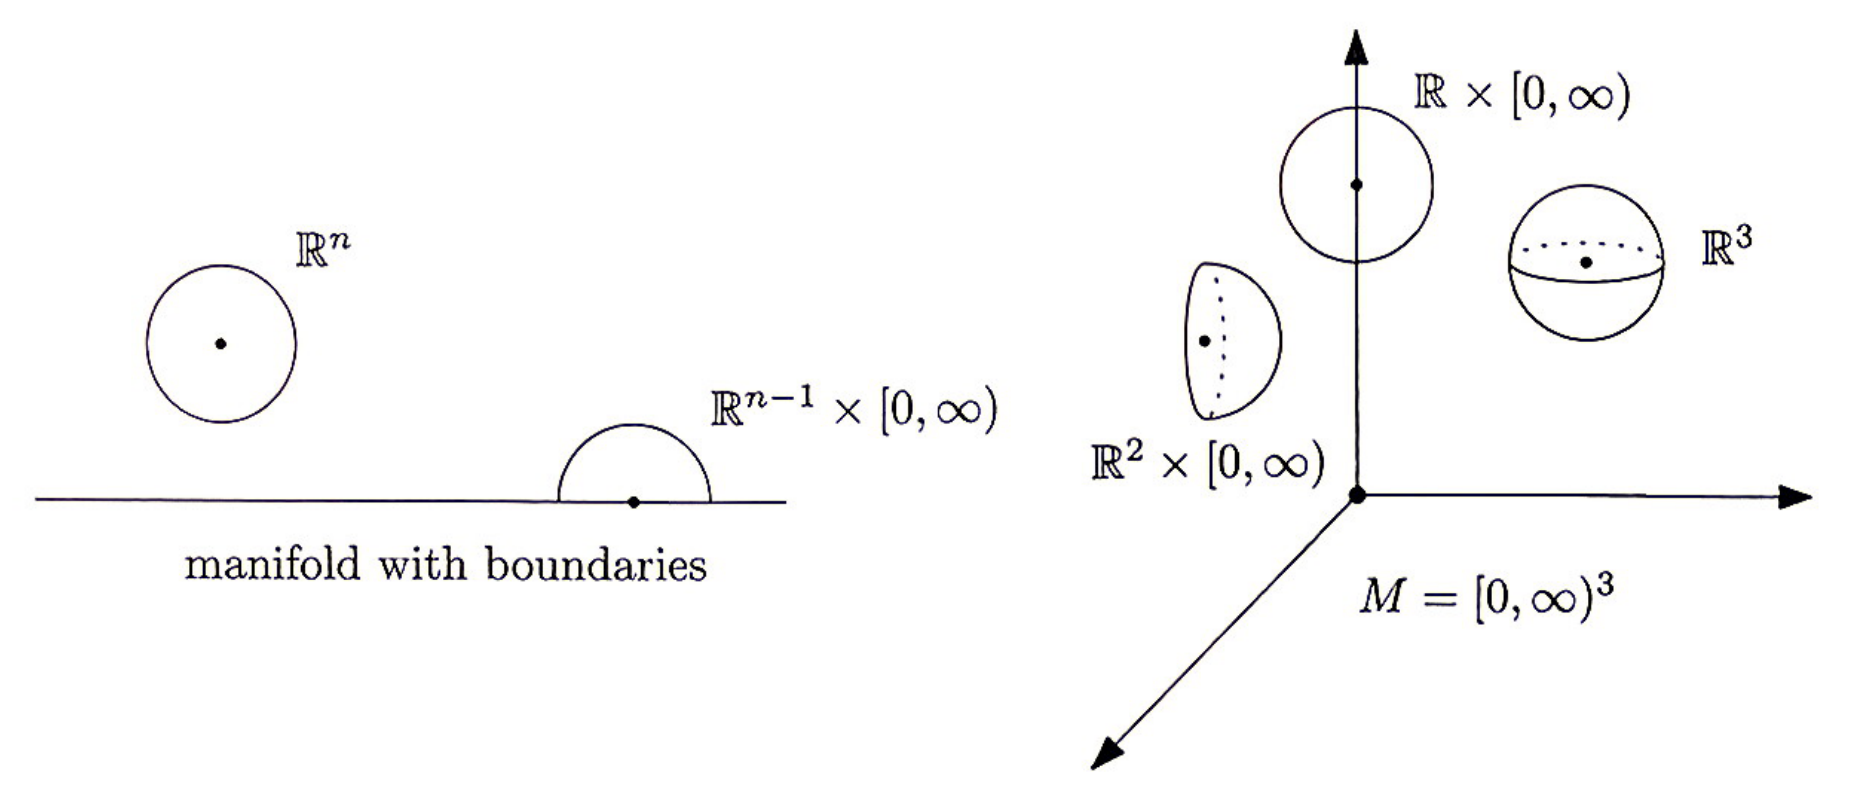
\includegraphics[width=0.9\linewidth]{figures/fig_p116_2.png}
  \caption*{图 5.6\quad 带角流形（原书 p.108, Figure 5.6；PDF p.116）}
\end{figure}

下面是一个标准例子。

\begin{wexam}{5.1.5}
考虑 $M=[0,\infty)^3$（即 $\R^3$ 中的闭象限）。除了经典的点
$p\in(0,\infty)^3$ 之外，还有一些「角」点。例如，点 $(1,0,1)\in M$ 在 $M$ 中有一个
邻域同胚于 $\R^2\times[0,\infty)$ 的某个开子集。再如，点 $(0,0,2)$ 在 $M$ 中有一个
邻域同胚于 $\R\times[0,\infty)^2$ 的某个开子集。另一个极端情形是点 $(0,0,0)$，它在
$M$ 中有一个邻域同胚于 $[0,\infty)^3$ 的某个开子集。

% >>> p117
我们可以导出 $M$ 的另一种几何结构。考虑 $M^{\mathrm{int}}:=(0,\infty)^3$，则它的
补集（在 $M$ 中）作为 $M$ 的闭子集，可以显式写出如下
\begin{equation}\tag{5.4}
M\setminus M^{\mathrm{int}}
=\left(\{0\}\times[0,\infty)^2\right)\cup
\left([0,\infty)\times\{0\}\times[0,\infty)\right)\cup
\left([0,\infty)^2\times\{0\}\right).
\end{equation}
于是 $M\setminus M^{\mathrm{int}}$ 中的每个连通分支都可以看成 $[0,\infty)^2$ 的一个
副本，而后者又有与 (5.4) 类似的分解。换言之，$M$ 具有一种「俄罗斯套娃」式的结构，
更专业的说法是 $M$ 的一个\textbf{分层}（stratification）。\hfill$//$
\end{wexam}

沿用例 5.1.5，让我们引入一些记号。给定带角流形 $M$，定义 $M$ 的
\textbf{余维 $k$ 分层}（codimension-$k$ stratum）为 $M$ 的如下开子集
\begin{equation}\tag{5.5}
M_k:=\left\{x\in M\ \middle|\
x\ \text{有一个邻域}\ U\cong V\subset\R^{n-k}\times[0,\infty)^k\right\}.
\end{equation}
在 $M$ 中取闭包，得到
\begin{equation}\tag{5.6}
\overline{M_k}=M_k\cup M_{k-1}\cup\cdots\cup M_n.
\end{equation}
换句话说，每个开子集 $M_k$ 都是 $M$ 的「积木」（building block）。例 5.1.5 中的讨论
可以改写成
\begin{equation}\tag{5.7}
\partial M:=M\setminus M_0=\overline{M_1}=M_1\cup M_2\cup\cdots\cup M_n,
\end{equation}
其中 $\partial M$ 称为 $M$ 的\textbf{边界}。注意，当 $M$ 只是（经典意义下的）光滑
带边流形时，(5.7) 中的 $\partial M$ 与 $M$ 的边界的标准记号一致（此时 (5.7) 中只出现
$M_1$ 这一项）。

% [Tutor Note: 易错预警——(5.6) 中闭包的指标顺序容易看反：$\overline{M_k}$ 含
% $M_k$ 以及\emph{更高}余维的分层 $M_{k-1},\cdots,M_n$（即角越尖，余维越大）。
% 因此 (5.7) 中 $\partial M=\overline{M_1}$ 是全部非内部点的并，而 $\overline{M_k}$
% 只有在 $k=1$ 时才等于边界。]

\begin{wrem}{5.1.2}
可能引起混淆的是：在某些文献中，闭包 $\overline{M_k}$ 也被称为（$M$ 的）余维 $k$
分层，而 $M_k$ 被称为余维 $k$ 的\emph{开}分层。
\end{wrem}

有了这些准备，我们就可以陈述 Morse 理论模空间中最重要的性质了。

\begin{wthm}{5.1.1}（[128] 中的定理 2.1）
给定闭流形 $X$ 及其上的通有 Morse 函数与度量对 $(F,g)$，对任意两个不同的
$x,y\in\Crit(F)$，由 (5.3) 定义的约化模空间
$\mathcal M(x,y)=\mathcal M_{F,g}(x,y)$ 具有一个紧化
$\overline{\mathcal M(x,y)}$，它是一个光滑带角流形。此外，其余维 $k$ 分层为
\begin{equation}\tag{5.8}
\overline{\mathcal M(x,y)}_k
=\bigcup_{x_1,\cdots,x_k\in\Crit(F)}
\mathcal M(x,x_1)\times\cdots\times\mathcal M(x_k,y),
\end{equation}
其中 $x,x_1,\cdots,x_k,y$ 是 $\Crit(F)$ 中互不相同的点。
\end{wthm}

% [Tutor Note: 含糊点拨——定理 5.1.1 的证明由两半组成：(1) \emph{紧性}：任何流线
% 序列在能量一致有界的条件下有收敛子列，其极限是断裂流线（这正是例 5.1.4 中
% 「$p_2\to q_1\to p_0$」型极限的推广）；(2) \emph{粘合}：把断裂流线在临界点处
% 「接上」，可在紧化空间中构造带角流形的局部模型 $\R^{n-k}\times[0,\infty)^k$。
% 这一紧化—粘合（compactness–gluing）模式在 5.4 节 Floer 理论中会原样出现，
% 只是分析难度大得多。]

用记号来说，$\overline{\mathcal M(x,y)}_k$ 与 (5.5) 中的 $M_k$ 是同一个东西。下面是
几个低维例子。

% >>> p118
\begin{wexam}{5.1.6}
当 $k=1$ 时，余维 $1$ 分层 $\overline{\mathcal M(x,y)}_1$ 中的每个元素都只有一个
中间点。因此其中的元素看起来就像图 5.7 所示的断裂流线。\hfill$//$
\end{wexam}

\begin{figure}[htbp]
  \centering
  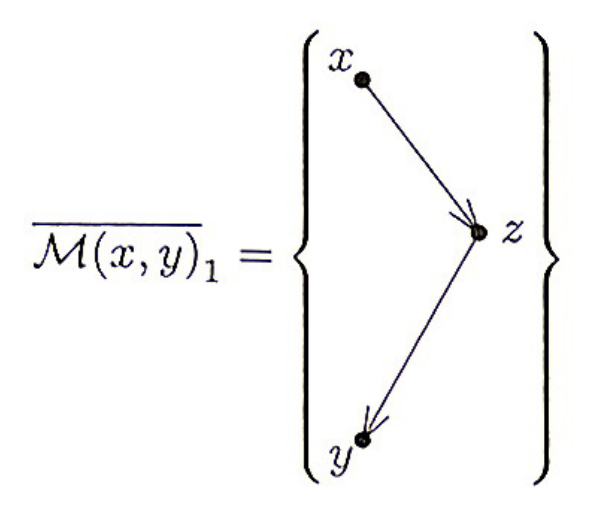
\includegraphics[width=0.32\linewidth]{figures/fig_p118_1.png}
  \caption*{图 5.7\quad $\overline{\mathcal M(x,y)}_1$ 中的元素（原书 p.110,
  Figure 5.7；PDF p.118）}
\end{figure}

\begin{wexam}{5.1.7}
设 $\overline{\mathcal M(x,y)}$ 具有一个 2-单形的结构（即一个二维带角流形），那么
它可以分解为图 5.8。\hfill$//$
\end{wexam}

\begin{figure}[htbp]
  \centering
  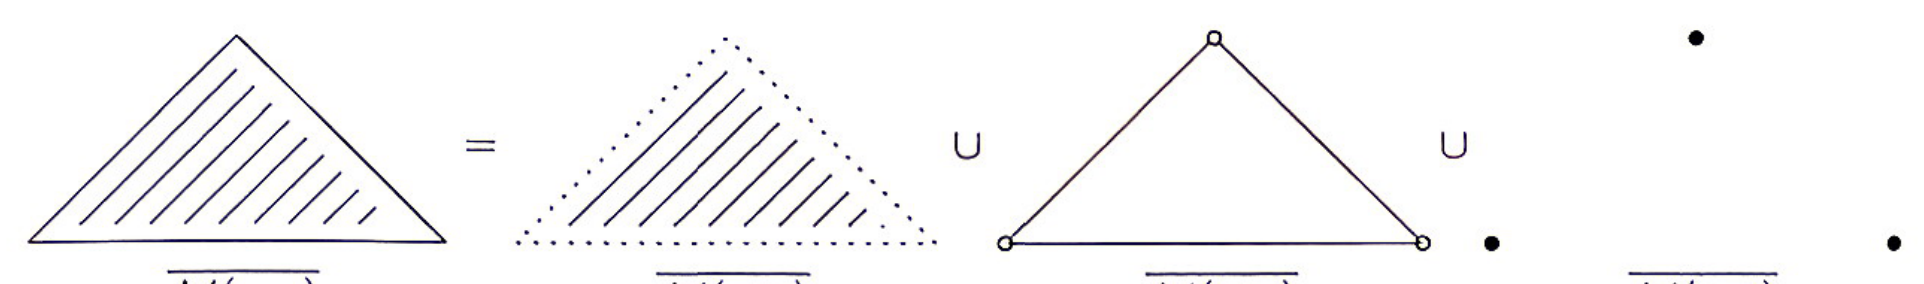
\includegraphics[width=0.95\linewidth]{figures/fig_p118_2.png}
  \caption*{图 5.8\quad $\overline{\mathcal M(x,y)}$ 按不同余维分层的分解（原书
  p.110, Figure 5.8；PDF p.118）}
\end{figure}

在定理 5.1.1 的情形中，关系 (5.6) 是这样实现的：$\overline{\mathcal M(x,y)}_1$ 的
闭包——用一个略显繁复的记号记作
$\overline{\overline{\mathcal M(x,y)}_1}$——如图 5.9 所示。此外，由 (5.7) 有
$\overline{\overline{\mathcal M(x,y)}_1}
=\partial\overline{\mathcal M(x,y)}$，因此图 5.9 也画出了
$\overline{\mathcal M(x,y)}$ 的边界。

\begin{figure}[htbp]
  \centering
  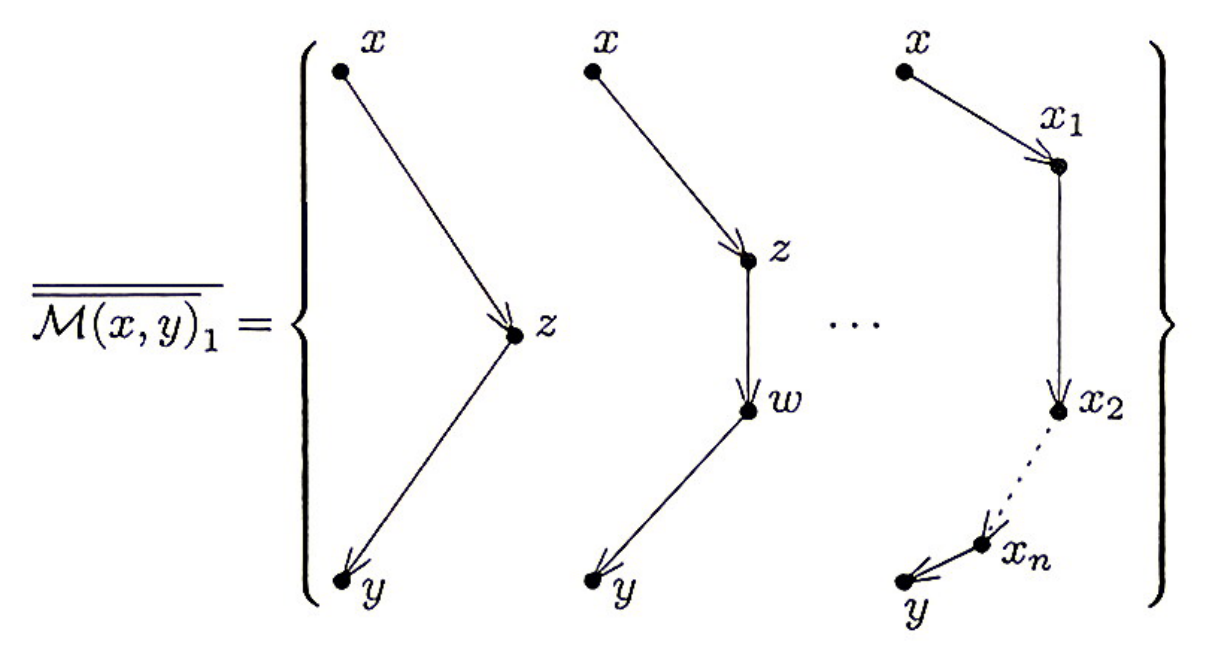
\includegraphics[width=0.62\linewidth]{figures/fig_p118_3.png}
  \caption*{图 5.9\quad $\overline{\mathcal M(x,y)}_1$ 的闭包，记作
  $\overline{\overline{\mathcal M(x,y)}_1}$（原书 p.110, Figure 5.9；PDF p.118）}
\end{figure}

% [Tutor Note: 易错预警——注意「套娃」式记号：$\overline{\mathcal M(x,y)}_1$ 表示
% $\overline{\mathcal M(x,y)}$ 的余维 $1$ 分层，再取闭包得到
% $\overline{\overline{\mathcal M(x,y)}_1}$，后者才等于 $\partial\overline{\mathcal M(x,y)}$。
% 这两个对象维数相同（都是 $\dim\overline{\mathcal M(x,y)}-1$），但前者是开分层、
% 后者是闭的带角流形；定理 5.1.1 的 (5.8) 描述的是后者的分层。]

% >>> p119
\begin{wexam}{5.1.8}（重要）
当 $\ind(x)-\ind(y)=1$ 时，情形会大大简化：此时 $\mathcal M(x,y)$ 已经是紧的，
且 $\dim\mathcal M(x,y)=0$（因为不会有中间点来构成断裂流线）。换言之，若
$\ind(x)-\ind(y)=1$，则
\[
\overline{\mathcal M(x,y)}=\mathcal M(x,y),\qquad
\partial\mathcal M(x,y)=\varnothing.
\]
结合命题 5.1.1 证明之后的结论 (ii)，我们知道 $\mathcal M(x,y)$ 将是一个由有限多个点
组成的集合（有限性来自紧性）。\hfill$//$
\end{wexam}

\begin{wexam}{5.1.9}
比例 5.1.8 稍复杂一些：若 $\ind(x)-\ind(y)=2$，则可能存在某些 $z\in\Crit(F)$
帮助构成断裂流线（如图 5.7，但只断裂一次！）。于是由 (5.7) 与定理 5.1.1，
\begin{align*}
\partial\overline{\mathcal M(x,y)}
&=\overline{\overline{\mathcal M(x,y)}_1}
=\overline{\mathcal M(x,y)}_1\cup\overline{\mathcal M(x,y)}_2\cup\cdots\\
&=\overline{\mathcal M(x,y)}_1\\
&=\bigcup_{z\in\Crit(F)}\mathcal M(x,z)\times\mathcal M(z,y).
\end{align*}
这尤其蕴含：边界 $\partial\overline{\mathcal M(x,y)}$ 是一个紧的一维流形（可能带边）。
由紧一维流形的分类，其边界分支（点）的个数总是偶数。\hfill$//$
\end{wexam}

% [Tutor Note: 易错预警——此例是整个构造的关键：$\ind(x)-\ind(y)=2$ 时，
% $\overline{\mathcal M(x,y)}$ 是一维带角流形，其边界点正是那些「一次断裂」的流线，
% 个数为偶数。这个偶性正是下一步证明 $\partial^2=0$ 的唯一输入。注意第三行
% $\overline{\mathcal M(x,y)}_2=\varnothing$？并非如此——它只是在上式中被并入了
% $\overline{\mathcal M(x,y)}_1$ 的闭包；原文写成等号是因为 (5.6) 已把更高余维分层
% 含在闭包中。]

\begin{wexer}{5.1.2}
考虑如下函数 $f:\C^{n+1}\setminus\{0\}\to\R$
\[
f(z_0,\cdots,z_n):=
\frac{\sum_{j=0}^{n}j|z_j|^2}{\sum_{j=0}^{n}|z_j|^2},
\qquad (z_0,\cdots,z_n)\in\C^{n+1}\setminus\{0\}.
\]
回忆 $\CP^n$ 可以构造为 $\C^{n+1}\setminus\{0\}$ 的商空间，其中
$(z_0,\cdots,z_n)\mapsto[z_0,\cdots,z_n]\in\CP^n$；于是上述 $f$ 下降为函数
$F:\CP^n\to\R$，定义为 $F([z_0,\cdots,z_n]):=f(z_0,\cdots,z_n)$。
\begin{enumerate}[label=(\roman*)]
  \item 证明 $F$ 是 $\CP^n$ 上的 Morse 函数。
  \item 求出 $F$ 的全部临界点并计算它们的指标。
  \item 描述维数最小的非零维数模空间 $\mathcal M(x,y)$。
\end{enumerate}
\end{wexer}

% [Tutor Note: 含糊点拨——此练习是 $\CP^n$ 上标准 Morse 函数（「高度函数」的复版本）
% 的计算：(ii) 的答案是临界点为坐标点 $[0:\cdots:1:\cdots:0]$，指标依次为
% $0,2,4,\cdots,2n$；(iii) 中最小非零维数的模空间对应于指标差 $2$（复维数差 $1$），
% 它是 $\CP^1$ 上的一个点（可用 $\CP^1$ 的显式流线验证）。这一例子在 8 章量子上同调
% 中会以「Clifford 环」的形式再次出现。]

Morse 理论的基本想法是把流形 $X$ 上的函数理论（Morse 函数的临界点）与代数
（同调理论）结合起来。有了上面引入的全部构件，我们就可以详细阐述这一点了。给定紧
流形 $X$ 与黎曼度量 $g$，我们按如下配方来构造 Morse 函数
$F:(X,g)\to\R$ 的所谓\textbf{Morse 同调}。

\textbf{第 1 步：构造 Morse 复形}（系数取 $\Z_2$）。令
\[
\mathrm{CM}_*(F,g;\Z_2):=\Z_2\langle x\in\Crit(F)\ \text{满足}\ \ind(x)=*\rangle,
\]
它首先是一个分次 $\Z_2$-模。

% >>> p120
$\mathrm{CM}_*(F,g;\Z_2)$ 中的元素是有限形式和
$\sum_{x\in\Crit(F)}a_x x$，其中 $a_x\in\Z_2$。

\textbf{第 2 步：定义 Morse 边界算子} $\partial_*$。在
$\mathrm{CM}_*(F,g;\Z_2)$ 上定义 $\Z_2$-线性映射
$\partial_*:\mathrm{CM}_*(F,g;\Z_2)\to\mathrm{CM}_{*-1}(F,g;\Z_2)$ 为
\[
x\mapsto
\sum_{\substack{y\in\Crit(F)\\ \ind(y)=*-1}}
\#_{\Z_2}\mathcal M(x,y)\,y.
\]
需要确认它确实是边界算子：对 $x\in\mathrm{CM}_*(F,g;\Z_2)$，按定义有
\begin{align*}
(\partial_{*-1}\circ\partial_*)(x)
&=\partial_{*-1}\left(
\sum_{\substack{y\in\Crit(F)\\ \ind(y)=*-1}}
\#_{\Z_2}\mathcal M(x,y)\,y\right)\\
&=\sum_{\substack{y\in\Crit(F)\\ \ind(y)=*-1}}
\#_{\Z_2}\mathcal M(x,y)\cdot
\left(\sum_{\substack{z\in\Crit(F)\\ \ind(z)=*-2}}
\#_{\Z_2}\mathcal M(y,z)\,z\right)\\
&=\sum_{\substack{z\in\Crit(F)\\ \ind(z)=*-2}}
\left(\sum_{\substack{y\in\Crit(F)\\ \ind(y)=*-1}}
\#_{\Z_2}\big(\mathcal M(x,y)\times\mathcal M(y,z)\big)\right)z\\
&=\sum_{\substack{z\in\Crit(F)\\ \ind(z)=*-2}}
\#_{\Z_2}\partial\overline{\mathcal M(x,z)}\,z=0,
\end{align*}
其中最后一个等号来自例 5.1.9 末尾关于模空间 $\partial\overline{\mathcal M(x,z)}$
之奇偶性的结论。这使得 $(\mathrm{CM}_*(F,g;\Z_2),\partial_*)$ 成为 $\Z_2$ 上的
一个良定义的链复形。

% [Tutor Note: 易错预警——此处系数取 $\Z_2$，故 $\#_{\Z_2}$ 只数「点的个数模 2」，
% 不需要考虑模空间的定向；换成一般系数时（见注 5.1.4），必须给模空间定向并计入
% 符号，否则 $\partial^2=0$ 不再成立。另注意 (5.8) 中乘积
% $\mathcal M(x,y)\times\mathcal M(y,z)$ 的粘合把两层断裂流线对应到
% $\partial\overline{\mathcal M(x,z)}$ 的边界点，这一步的严格性依赖定理 5.1.1 的
% 带角流形结构。]

\textbf{第 3 步：定义 Morse 同调群}。按由链复形定义同调群的通常方式，考虑
\begin{equation}\tag{5.9}
\mathrm{HM}_*(F,g;\Z_2):=
\frac{\ker\left(\partial_*:\mathrm{CM}_*(F,g;\Z_2)
\to\mathrm{CM}_{*-1}(F,g;\Z_2)\right)}
{\operatorname{im}\left(\partial_{*+1}:\mathrm{CM}_{*+1}(F,g;\Z_2)
\to\mathrm{CM}_*(F,g;\Z_2)\right)}.
\end{equation}
这些是分次 $\Z_2$-模，从记号上看依赖于 Morse 函数 $F$ 与 $X$ 上的度量 $g$。

\begin{wrem}{5.1.3}
严格说来，由于我们在第 2 步中使用了定理 5.1.1 的性质（更确切地说，是其中的紧化与
分层结构），度量 $g$ 应当通有地选取。
\end{wrem}

下面这个结果是 Morse 理论的核心定理，它证明上面定义的
$\mathrm{HM}_*(F,g;\Z_2)$ 实际上是流形 $X$ 本身的拓扑不变量。

% >>> p121
\begin{wthm}{5.1.2}（[199] 中的定理 8.9）
给定紧流形 $X$，对 $X$ 上任意两对通有的 Morse 函数与度量 $(F,g)$ 与 $(F',g')$，
有
\[
\mathrm{HM}_*(F,g;\Z_2)\cong\mathrm{HM}_*(F',g';\Z_2),
\]
其中 $\Z_2$ 为任意域。此外，$\mathrm{HM}_*(F,g;\Z_2)\cong H_*(X;\Z_2)$，即 $X$ 的
经典同调群（$\Z_2$ 系数）。
\end{wthm}

% [Tutor Note: 原文疑误（表述）——定理中「for any field $\Z_2$」的措辞不严谨：
% $\Z_2$ 已经固定，不能同时又「任意」。结合注 5.1.4 可知作者本意是「对任意系数域
% $\mathbf k$ 成立」。译文照原文译出并在此说明，详见 review_ch05a.md。]

% [Tutor Note: 含糊点拨——两种 Morse 函数与度量之间的同构通常通过「延拓映射」
% （continuation map）证明：在 $X\times[0,1]$ 上取一族从 $(F,g)$ 到 $(F',g')$ 的
% 插值，数一族含参数流线（即「$1$ 维模空间」），再证明其诱导映射与参数无关且可逆。
% 这一手法在 5.4 节 Floer 理论中称为 Floer 延拓映射，是 Floer 同调良定义性的
% 标准论证。]

\begin{wrem}{5.1.4}
定理 5.1.2 的同一结论对任意系数 $\mathbf k$ 成立。唯一的区别在于：验证上面的第 2 步
时，最后一步
$\sum\#_{\Z_2}\partial\overline{\mathcal M(x,z)}\,z=0$（每当
$\ind(x)-\ind(z)=2$）需要对模空间的定向额外小心。更多细节见 [132] 的 6.6 节。
\end{wrem}

由于定理 5.1.2 与注 5.1.4，我们把一般系数 $\mathbf k$ 下的 Morse 同调记作
$\mathrm{HM}_*(F,g;\mathbf k)$；若无需强调度量 $g$，则更简略地记作
$\mathrm{HM}_*(F;\mathbf k)$。

定理 5.1.2 的一个直接应用，是给出同时证明闭流形上 Poincaré 对偶与 Künneth 公式的
工具。

\begin{wexer}{5.1.3}
应用定理 5.1.2 证明下列结果。
\begin{enumerate}[label=(\roman*)]
  \item （Poincaré 对偶）$H_*(M;\mathbf k)\cong H_{\dim M-*}(M;\mathbf k)$；
  \item （Künneth 公式）
        $H_*(M\times N;\mathbf k)\cong
        \bigoplus_{i+j=*}H_i(M;\mathbf k)\otimes H_j(N;\mathbf k)$，
\end{enumerate}
其中 $\mathbf k$ 是域，可安全地取为 $\Z_2$。
\end{wexer}

定理 5.1.2 的另一个应用，是导出光滑流形上 Morse 函数的某些刚性。具体地说，对 $X$
（$n$ 维光滑流形）上的任意 Morse 函数 $F$，有
\begin{align*}
\#\Crit(F)
&=\sum_{i=0}^{n}\dim_{\mathbf k}\mathrm{CM}_i(F,g;\mathbf k)\\
&\geqslant\sum_{i=0}^{n}\dim_{\mathbf k}\mathrm{HM}_i(F,g;\mathbf k)
=\sum_{i=0}^{n}\dim_{\mathbf k}H_i(X;\mathbf k)
=\sum_{i=0}^{n}b_i(X;\mathbf k),
\end{align*}
其中 $b_i(X;\mathbf k)$ 是 $X$ 的第 $i$ 个 Betti 数（系数在 $\mathbf k$ 中）。作为
具体例子，在 2-环面 $\T^2$ 上，任意 Morse 函数在 $\T^2$ 上至少须有 $4$ 个临界点，
因为 $\sum_{i=0}^{2}b_i(\T^2;\mathbf k)=4$（参见例 5.1.4）。

% [Tutor Note: 易错预警——上面不等式链的第一个「$\geqslant$」用的是
% $\dim\ker\partial_i\geqslant\dim H_i$ 以及 $\#\Crit(F)=\sum_i\dim\mathrm{CM}_i$；
% 第二个等号用定理 5.1.2。这就是 Morse 不等式（Morse inequalities）的弱形式；
% 逐项加强可得到 $\sum_{i\leqslant j}(-1)^{j-i}\#\Crit_i\geqslant
% \sum_{i\leqslant j}(-1)^{j-i}b_i$。]

在结束本节之前，让我们回到例 5.1.3 中的心形圆周（作一点变形），计算其 Morse 同调群，
并验证定理 5.1.2。

\begin{wexam}{5.1.10}
考虑心形圆周 $X$ 上的高度函数 $F$（见图 5.10）。沿用上面的步骤，我们来计算与这个
高度函数 $F$ 相联系的 Morse 同调群。由于度量 $g$ 总取从 $\R^2$ 诱导的标准度量，
为简洁起见，把所得的 $\mathbf k$-模记作 $\mathrm{CM}_*(F;\mathbf k)$。与例
% >>> p122
5.1.2 类似，仅有的非平凡 $\mathbf k$-模如下
\[
\mathrm{CM}_0(F;\mathbf k)=\mathbf k\langle p_0,q_0\rangle,
\qquad
\mathrm{CM}_1(F;\mathbf k)=\mathbf k\langle p_1,q_1\rangle.
\]
于是唯一非零的 Morse 边界算子是
$\partial_1:\mathrm{CM}_1(F;\mathbf k)\to\mathrm{CM}_0(F;\mathbf k)$，定义为
\[
p_1\mapsto p_0+q_0,\qquad q_1\mapsto p_0+q_0,
\]
它来自对负梯度流线的计数。特别地，$\partial_0=\partial_2=0$。为后文（见 5.2 节）
方便，我们为 $\mathrm{CM}_0(F;\mathbf k)$ 与 $\mathrm{CM}_1(F;\mathbf k)$ 另选一组基，
明确写出如下
\[
\mathrm{CM}_0(F;\mathbf k)=\mathbf k\langle p_0,e\rangle,
\qquad
\mathrm{CM}_1(F;\mathbf k)=\mathbf k\langle p_1,f\rangle,
\]
其中 $e=p_0+q_0$，$f=p_1-q_1$。在这组基下，有
$\partial_1p_1=e$ 与 $\partial_1f=0$。于是计算 Morse 同调群，得到
\begin{equation}\tag{5.10}
\begin{aligned}
\mathrm{HM}_0(F;\mathbf k)
&=\ker(\partial_0)/\operatorname{im}(\partial_1)
=\mathbf k\langle p_0,e\rangle/\mathbf k\langle e\rangle
\cong\mathbf k\langle p_0\rangle,\\
\mathrm{HM}_1(F;\mathbf k)
&=\ker(\partial_1)/\operatorname{im}(\partial_2)
=\mathbf k\langle f\rangle/0\cong\mathbf k\langle f\rangle.
\end{aligned}
\end{equation}
这些与 $\R^2$ 中圆周的经典同调群一致。\hfill$//$
\end{wexam}

\begin{figure}[htbp]
  \centering
  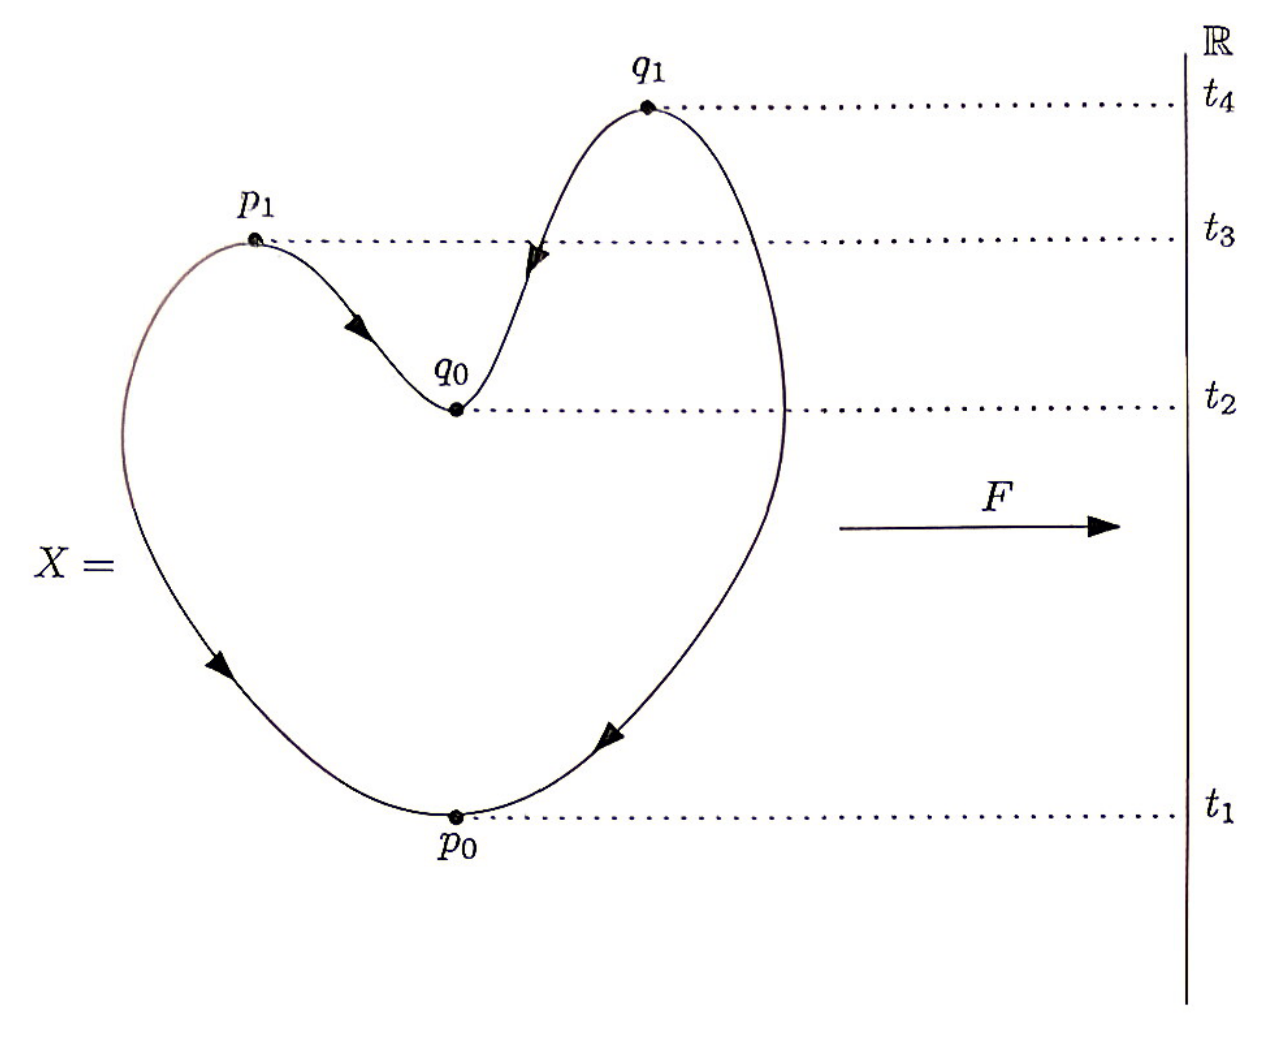
\includegraphics[width=0.68\linewidth]{figures/fig_p122_1.png}
  \caption*{图 5.10\quad 临界值互不相同的高度函数（原书 p.114, Figure 5.10；
  PDF p.122）}
\end{figure}

% [Tutor Note: 易错预警——(5.10) 中第一个分式
% $\mathbf k\langle p_0,e\rangle/\mathbf k\langle e\rangle$ 的分子是
% $\mathrm{CM}_0$ 的\emph{基}生成的子模，不要与 $\ker\partial_0=\mathrm{CM}_0$
% 弄混；$\partial_0=0$ 故 $\ker\partial_0=\mathrm{CM}_0$，于是商掉
% $\operatorname{im}\partial_1=\mathbf k\langle e\rangle$。另注意
% $f=p_1-q_1$ 满足 $\partial_1f=0$，这正是 $f$ 在 $\mathrm{HM}_1$ 中给出非平凡类
% 的原因。]

为结束本节，让我们把 Morse 理论的优点总结如下。
\begin{enumerate}[label=(\roman*)]
  \item 它以相当可计算的方式恢复所在流形的拓扑，因为我们可以相当灵活地选取 Morse
        函数（见事实 5.1.2）。
  \item 可以把本节中的 Morse 理论推广到无穷维情形，这是 Floer 理论的强有力动机
        （见 5.4 节）。
% >>> p123
  \item 从 Morse 同调群的构造中我们获得了额外信息：任意 $x\in\Crit(F)$ 天然带有
        一个值 $F(x)$。注意，在本节的构造中 $\mathrm{HM}_*(F,g;\mathbf k)$ 并未
        用到这一信息。下一节我们将看到如何改进这一点。
\end{enumerate}

% [Tutor Note: 含糊点拨——第 (ii) 条所说的「无穷维情形」需要克服两类困难：其一，
% 环路空间/道路空间不是有限维流形，需用 Fredholm 理论定义「指标」；其二，
% 无穷维中模空间的横截性一般不成立（存在「泡泡」等紧性障碍），这正是伪全纯曲线
% 理论的工作所在。5.4 节会给出正式的哈密顿 Floer 理论。]
